\ifsolo
~

\vspace{1cm}

\begin{center}
    \textbf{\LARGE Calcul différentiel} \\[1em]
\end{center}
\tableofcontents
\else
\minitoc
\fi
\thispagestyle{empty}

\ifsolo \newpage \setcounter{page}{1} \fi
\section{Notions, Définitions}

$E$ est un $\mathbb R$-e.v de dimension $n$ (donc isomorphe à $\mathbb R^n$), $F$ un sev de $E$ et $\Omega$ un ouvert de $E$.

\begin{rem}
    Pour $a\in\Omega, v\in E, \exists \epsilon>0, \forall t\in ]-\epsilon, \epsilon[, a+tv\in\Omega$ (par définition d'un ouvert)
\end{rem}

\begin{dfn}
    On note $f:\Omega \longrightarrow F$. On dira que $f$ possède une dérivée\index{dérivée partielle} en $a\in\Omega$ selon $v\in E$ si \[
        \lim_{\substack{t\to 0\\ t\neq 0}}\frac{f(a+tv)-f(a)}t
    \] existe. On note cette limite $D_vf(a)$.

    Si $\mathcal B=(e_1,\cdots, e_n)$ base de $E$ et $f$ a une dérivée en $a\in\Omega$ selon $e_{i_0}$ alors on appelle $i_0$-ième dérivée partielle $D_{e_{i_0}}f(a)$, notée \[
        \frac{\partial f}{\partial x_{i_0}}(a)\qquad \text{ ou }\qquad \partial_{i_0}f(a)
    \]
\end{dfn}

\begin{rem}
    Pour $\mathcal B=(e_1, \cdots, e_n)$ on note $x\underset{\mathcal B}{\longleftrightarrow}(x_1, \cdots, x_n)$ et on a $f(x)=f(x_1e_1+\cdots + x_ne_n)$ qu'on note abusivement $f(x_1, \cdots, x_n)$. \[
        \frac{f(x+te_1)-f(x)}{t}=\frac{f(x_1+t, x_2, \cdots, x_n)-f(x_1, \cdots, x_n)}{t}
    \]
    Pour calculer $\partial_if(a)$, on fait comme si les autres variables étaient constantes et on dérive par rapport à $x_i$.
\end{rem}

\begin{rem}
    $D_v$ est linéaire
\end{rem}

\begin{rem}
    Avoir une dérivée en $a$ n'implique pas la continuité en $a$. Contre-exemple: \[
        f(x, y)=\begin{cases}
            \frac{y^2}x &\text{ si }x\neq 0\\ y & \text{ sinon}
        \end{cases}
    \]
\end{rem}

\section{Différentielle}

\begin{defprop}
    \Hyp $f:\Omega\longrightarrow F$, $a\in \Omega$. \begin{concenum}
    \item On dira que $f$ est différentiable\index{différentielle} en $a$ s'il existe $\varphi\in\mathcal L(E, F), \epsilon>0$ tels que \[
            \forall h\in\mathcal B_o(0, \epsilon), f(a+h)=f(a)+\varphi(h)+o_0(h)
        \]
        Dans ce cas $\varphi$ est unique et se note $\diff f_a$
    \item Si $f$ est différentiable en $a$ alors $f$ est continue en $a$
    \item Si $f$ est différentiable en $a$ alors $f$ a une dérivée en $a$ selon tout $v$ et \[
            D_vf(a)=df_a(v)
        \]
    \end{concenum}
\end{defprop}

\begin{proof} ~
    \begin{enumerate}
        \item Si $\varphi, \psi$ conviennent, $\varphi(tv)-\psi(tv)=o_0(tv)$ ie \[
                \varphi(v)-\psi(v)=o_0(v)\xrightarrow[t\to 0]{}0
            \]
            d'où $\varphi\equiv \psi$.
        \item $f(a+h)=f(a)+\varphi(h)+o_0(h)\xrightarrow[h\to 0]{}f(a)$
        \item \[
                \frac{f(a+tv)-f(a)}{t}=\diff f_a(v)+o_0(v)\xrightarrow[\substack{t\to 0\\t\neq 0}]{}\diff f_a(v)
            \]
    \end{enumerate}
\end{proof}

\begin{thmdef}
    ~ \begin{enumerate}
        \item Soit $f\in\mathcal L(E, F)$ et $a\in E$. La fonction $f$ est différentiable en $a$ et $df_a=f$.
        \item Si $\mathcal B=(e_1, \cdots, e_n)$ est une base de $E$ et si $\pi_i$ est l'application $i$-ième coordonnée alors $\forall a\in E, \diff \pi_i=\pi_i$ se dépend pas de $a$. On note cette application $\diff x_i$.
        \item Si $\mathcal B$ est une base de $E$ et $f$ est différentiable en $a$ alors \[
                \diff f_a=\sum_{i=1}^n\frac{\partial f}{\partial x_i}(a)\diff x_i
            \]
    \end{enumerate}
\end{thmdef}

\begin{proof} ~
    \begin{enumerate}
        \item $f(a+h)=f(a)+f(h)$
        \item Ok
        \item $h=h_1e_1+\cdots +h_ne_n$, \[
                \diff f_a(h)=h_1\diff f_a(e_1)+\cdots +h_n\diff f_a(e_n)=\sum_{i=1}^n\frac{\partial f}{\partial x_i}(a)\diff x_i
            \]
    \end{enumerate}
\end{proof}

\begin{rem}
    Pour une fonction $f:\mathbb R\longrightarrow F$, $f'(a)=\diff f_a(1)$
\end{rem}

\section{Calculs de différentielles}

\subsection{Quelques exemples}
\begin{ex} Étude en $0$ de
    \[
        f(x, y)=\begin{cases}
            \frac{y^2}x &\text{ si }x\neq 0\\ y & \text{ sinon}
        \end{cases}
    \]
\end{ex}

\[
    \frac{\partial f}{\partial x}(0, 0)=0 \qquad\qquad \frac{\partial f}{\partial y}(0, 0)=f(0, 1)=1
\]
donc \[
    \frac{\partial f}{\partial x}(0, 0) \diff x+ \frac{\partial f}{\partial y}(0, 0)\diff y
\]
existe mais $f$ est non différentiable car non $\mathcal C^0$

\begin{ex} Calcul de la différentielle de
    {$f:A\in\mathcal M_n(\mathbb R)\longmapsto A^2$}
\end{ex}

\[
    f(A+H)=f(A)+AH+HA+H^2
\]
et pour une norme sous-multiplicative, $\|H^2\|\leq \|H\|^2=o_0(H)$ donc \[
    \diff f_A(H)=AH+HA
\]

\begin{ex} Calcul de la différentielle de
    {$f:M\in GL_n(\mathbb R)\longmapsto M^{-1}$}
\end{ex}

On fixe $M\in GL_n(\mathbb R)$. Alors $\exists \epsilon >0 / \mathcal B_o(M, \epsilon)\subset GL_n(\mathbb R)$. Pour $H$ dans $\mathcal B_o(0, \epsilon)$, \[
    M+H\in\mathcal B_o(M, \epsilon)
\]
et \[
    \left((M+H)^{-1}-M^{-1}\right)(M+H)=I_n-M^{-1}(M+H)=-M^{-1}H
\] donc
\begin{align*}
    (M+H)^{-1}-M^{-1}&=-M^{-1}H(M+H)^{-1}\\&=-M^{-1}HM^{-1}+M^{-1}Ho_0(1)\\&=\underbrace{-M^{-1}HM^{-1}}_{\diff f_M(H)}+o_0(H)
\end{align*}

\begin{exo} Calcul de la différentielle de
    {$f:A\in\mathcal M_n(\mathbb R)\longmapsto A^\intercal A$}
\end{exo}

\needspace{5\baselineskip}
\subsection{Interprétation matricielle}

\begin{thmdef}
    On note $f:\Omega\to \mathbb R^m$, $\Omega\subset \mathbb R^n$, on écrit $f=(f_1, \cdots, f_m)$. On suppose que $f$ est différentiable en $a\in\Omega$ et on note $\mathcal C_n$ (resp. $\mathcal C_m$) la base canonique de $\mathbb R^n$ (resp. $\mathbb R^m$). Alors: \begin{enumerate}
        \item On appelle matrice jacobienne\index{jacobienne (matrice -- )} de $f$ en $a$ la matrice \[
                J_f(a)=\left(\frac{\partial f_i}{\partial x_j}(a)\right)_{\substack{1\leq i\leq n\\ 1\leq j\leq n}}
            \]
        \item Si $x\underset{\mathcal C_n}{\longleftrightarrow}X$ alors \[
                \diff f_a(x)\underset{\mathcal C_m}\longleftrightarrow J_f(a)X
            \]
    \end{enumerate}
\end{thmdef}

\begin{proof}
    \[
        \diff f_a(x)=\sum_{i=1}^n\underbrace{\frac{\partial f}{\partial x_i}(x)}_{\displaystyle \left(\frac{\partial f_1}{\partial x_i}(x), \cdots, \frac{\partial f_m}{\partial x_i}(x)\right)}\overbrace{\diff x_i(x)}^{=x_i} \qquad \underset{\mathcal C_n}{\longleftrightarrow}\qquad \begin{pmatrix}
            \sum_{i=1}^n\limits \frac{\partial f_1}{\partial x_i}(a)x_i \\
            \vdots \\
            \sum_{i=1}^n\limits \frac{\partial f_m}{\partial x_i}(a)x_i
        \end{pmatrix}=J_f(a)X
    \]
\end{proof}

\section{Opérations sur les différentielles}

\begin{prop}
    Si $f,g:\omega\subset E\to F$ sont différentiables en $a$, alors pour $\lambda\in\mathbb R$, $\lambda f+g$ est différentiable en $a$ et $\diff (\lambda f+g)_a=\lambda df_a+\diff g_a$ \index{différentielle!opérations}
\end{prop}

\begin{prop}
    \Hyp $B:E_1\times E_2\to F$ bilinéaire, $f_1:\Omega_1\to E_1$ différentiable en $a_1$, $f_2:\Omega_2\to E_2$ différentiable en $a_2$.
    \Conc $f=B(f_1, f_2)$ est différentiable en $a=(a_1, a_2)$ et \[\diff f_a(h_1, h_2)=B(\diff {f_1}_{a_1}(h_1), f_2(a_2))+B(f_1(a_1), \diff {f_2}_{a_2}(h_2)) \]
\end{prop}

\begin{proof}
    On développe $f(a+h)=B(f_1(a_1+h_1), f_2(a_2+h_2))$
\end{proof}

\begin{ex} ~
    \begin{itemize}
        \item $(E, (\; |\; ))$ euclidien, $\varphi:(x, y)\longmapsto (x|y)$ \[
                \diff \varphi_{(x, y)}(h, k)=(h|y)+(x|k)
            \]
        \item $\varphi = \det $. On note \[
                A = (C_1 \cdots C_n) \quad H=(H_1 \cdots H_n)
            \]
            alors \[
                \det(A+H)=\det(A)+\det(H_1, C_2, \cdots, C_n)+\cdots + \det(C_1, \cdots, C_{n-1}, H_n)+o_0(H)
            \]
            On en déduit \begin{align*}
                \diff \varphi_A(H) &= \sum_{j=1}^n \det(C_1, \cdots, H_i, \cdots, C_n)\\
                                   &= \sum_{j=1}^n\sum_{i=1}^n(-1)^{i+j}h_{i, j}\Delta_{i, j}(A) \\
                                   &= \Tr(\Com(A)^\intercal H)
            \end{align*}
    \end{itemize}
\end{ex}

\section{Composition des fonctions différentielles}

\begin{prop}
    \Hyp $f : \Omega \subset E \to F$ différentiable en $a$ telle que $f(\Omega)\subset \Omega'$, $g : \Omega'\subset F \to G$ différentiable en $f(a)$
    \Conc $g\circ f$ est différentiable en $a$ et $\diff (g\circ f)_a=\diff g_{f(a)}\circ \diff f_a$ \index{différentielle!composition}
\end{prop}

\begin{proof}
    On a \[
        g(f(a)+k)=g(f(a))+\diff g_{f(a)}(k)+o(k)
    \]
    et \[
        f(a+h)=f(a)+\underbrace{\diff f_a(h)+o(h)}_{k}
    \]
    donc \[
        g\circ f(a+h)=g(f(a))+\diff g_{f(a)}(\diff f_a(h)+o_0(h)) + \underbrace{o(\underbrace{\diff f_a(h)+o_0(h)}_{o(h)})}_{o(h)}
    \]
    d'où \conc
\end{proof}

\begin{rem}
    $E=\mathbb R^n$, $F=\mathbb R^m$, $G=\mathbb R^p$, $f=(f_1, \cdots, f_m):E\to F$, $g=(g_1, \cdots, g_p):F\to G$, $\mathcal C_k$ base canonique de $\mathbb R^k$.

    Si $x \underset{\mathcal C_n}\longleftrightarrow X$ alors $\diff f_a(x)\underset{\mathcal C_m}\longleftrightarrow J_f(a)X$ et $\diff (g\circ f)_a(x)\underset{\mathcal C_p}\longleftrightarrow J_{g\circ f}(a)X\underset{\mathcal C_p}\longleftrightarrow J_g(f(a))J_f(a)X$. C'est vrai pour tout $X$ donc \[
        \underbrace{J_{g\circ f}(a)}_{\in\mathcal M_{p,n}} = \underbrace{J_g(f(a))}_{\in\mathcal M_{p,m}}\underbrace{J_f(a)}_{\in \mathcal M_{m,n}}
    \]
    On va identifier le coefficient $i, j$. \begin{align*}
        & \left[ J_{g\circ f}(a) \right]_{i, j}=\sum_{k=1}^m \left[ J_g(f(a)) \right]_{i, k} \left[ J_f(a) \right]_{k, j} \\
        \iff & \frac{\partial (g_i\circ f)}{\partial x_j} (a)=\sum_{k=1}^m \frac{\partial g_i}{\partial y_k}(f(a)) \frac{\partial f_k}{\partial x_j} (a) \\
        \iff & \colorboxed{red}{\partial_j (g_i\circ f)(a)=\sum_{k=1}^m\partial_kg_i(f(a))\partial_jf_k(a)} \quad \text{ \emph{(règle de la chaîne)} }
    \end{align*}

    En particulier, si $p = n = 1$, $\varphi:t\in \mathbb R\to g(f_1(t), \cdots, f_m(t))$ alors \[
        (g\circ f)'(a)=\sum_{k=1}^m \frac{\partial g}{\partial y_k}(f(a))f'_k(a)
    \]
\end{rem}

\begin{rem}
    Si $f:\Omega\subset E\to \mathbb R$ est différentiable en $a$ et $f(a)\neq 0$ alors $\frac 1f$ est différentiable en $a$ car $x\longmapsto \frac 1x$ est différentiable en $f(a)$
\end{rem}

\begin{rem}
    Si $f:\Omega\subset E\to F$ est $a\in\Omega$, $v\in E$ alors $\varphi:t \longmapsto f(a+tv)$ est définie au $\mathcal V(0)$ et $\varphi'(t)=\diff f_{a+tv}(v)$
\end{rem}

\needspace{5cm}
\section{Applications de classe \texorpdfstring{$\mathcal C^1$}{C1}}

\begin{thmdef}
    \Hyp $f:\Omega\subset E\longrightarrow F$
    \begin{concenum}
    \item On dira que $f$ est $\mathcal C^1$ sur $\Omega$ si $f$ est différentiable sur $\Omega$ et si $a\in\Omega \longmapsto \diff f_a\in\mathcal L(E, F)$ est $\mathcal C^0$
    \item Une fonction $\mathcal C^1$ est continue
    \item On note $\mathcal B=(e_1, \cdots, e_n)$ une base de $E$, $\mathcal C=(u_1, \cdots, u_m)$ une base de $F$ et $f=(f_1, \cdots, f_m)$. Il y a équivalence entre: \begin{enumerate}
        \item $f$ est $\mathcal C^1$ sur $\Omega$
        \item Les $f_i$ ont toutes leurs dérivées partielles sur $\Omega$ et les $\partial_jf_i$ sont $\mathcal C^0$ sur $\Omega$
    \end{enumerate}
\item On note $\mathcal C^1(\Omega, F)$ l'ensemble de ces fonctions
\end{concenum}
\end{thmdef}

\begin{proof}~
    \begin{enumerate}
        \setcounter{enumi}{1}
    \item Les fonctions $\mathcal C^1$ sont différentiables donc continues.
    \item $(a) \implies (b)$: \[
            J_f(a)=\mathcal M_{\mathcal B, \mathcal C}(\diff f_a)= \left( \frac{\partial f_i}{\partial x_j} (a) \right)_{\substack{1\leq i\leq m\\1\leq j\leq n}}
        \]
        est continue par rapport à $a$ par hypothèse.

        $(b) \implies (a)$: Il suffit de montrer que $f$ est différentiable sur $\Omega$. On commence par le cas $F=\mathbb R$. \begin{align*}
            f(a+h)-f(a) = \phantom{+} & f(a_1+h_1, \cdots, a_n+h_n)-f(a_1, a_2+h_2, \cdots, a_n+h_n) \\
            + & f(a_1, a_2+h_2, \cdots, a_n+h_n)-f(a_1, \cdots, a_i, a_{i+1}+h_{i+1}, \cdots, a_n+h_n) \\
            + & f(a_1, \cdots, a_i, a_{i+1}+h_{i+1}, \cdots, a_n+h_n) + \cdots \\
            + & f(a_1, \cdots, a_{n-1}, a_n+h_n)-f(a_1, \cdots, a_n)
        \end{align*}
        et chaque ligne est fonction d'une seule variable, donc le théorème des accroissements finis donne
        \begin{align*}
            \exists c_{i,h}\in]a_i,a_i+h_i[, \quad f(a+h)-f(a)=\phantom+ &
            h_1\frac{\partial f}{\partial x_1}(c_{1,h}, a_2+h_2, \cdots, a_n+h_n)\\
            + & h_2 \frac{\partial f}{\partial x_2}(a_1, c_{2,h},a_3+h_3,\cdots, a_n+h_n)\\
            + & \hspace{2cm}\vdots \\
            + & \underbrace{h_n \frac{\partial f}{\partial x_n} (a_1, \cdots, a_{n-1}, c_{n,h})}_{\longrightarrow h_n \frac{\partial f}{\partial x_n}(a) \text{ donc } =h_n \frac{\partial f}{\partial x_n}(a)+o(1) } \\
            =\phantom + & \underbrace{h_1 \frac{\partial f}{\partial x_1}(a)+\cdots + h_n \frac{\partial f}{\partial x_n} (a) }_{\text{AL}}  + \underbrace{h_1o(1)+\cdots h_no(1)}_{o(h)}
        \end{align*}
        donc $f$ est différentiable sur $\Omega$. Si $F\neq R$ on raisonne coordonnée par coordonnée.
\end{enumerate}
\end{proof}

\begin{prop} ~
    \begin{enumerate}
        \item $\mathcal C^1(\Omega, F)$ est un $\mathbb R$-e.v.
        \item Si $\mathcal C$ base de $F$ est $f:\Omega\longrightarrow F$ donnée par $f=(f_1, \cdots, f_n)$ (dans $\mathcal C$) alors il y a équivalence entre \begin{enumerate}
            \item $f$ est $\mathcal C^1$
            \item Les $f_i$ sont toutes $\mathcal C^1$
        \end{enumerate}
    \item Si $f:\Omega\longrightarrow F$ et $g: \Omega'\supset f(\Omega)\longrightarrow G$ sont $\mathcal C^1$ alors $g\circ f$ aussi
\end{enumerate}
\end{prop}

\begin{proof}
    1. et 2. sont faciles, 3. est déjà vu.
\end{proof}

\begin{thm}
    \Hyp $f:\Omega\subset E\longrightarrow \mathbb R$, $a,b\in\Omega$ tels que $[a, b]\subset \Omega$
    \begin{concenum}
    \item \[ f(b)-f(a)=\int_0^1\mathrm df_{(1-t)a+tb}(b-a)\diff t\]
    \item Si $\nop \diff f_x\nop\leq M$ pour $x\in[a, b]$ alors $|f(b)-f(a)|\leq M\|b-a\|$
    \end{concenum}
\end{thm}

\begin{proof}
    \begin{enumerate}
        \item $\varphi:t\longmapsto f(a+t(b-a))$ est telle que $\varphi'(t)=df_{(1-t)a+tb}(b-a)$ et \[
                f(b)-f(a)=\varphi(1)-\varphi(0)=\int_0^1\varphi'
            \]
        \item \[
                |f(b)-f(a)|\leq \int_0^1\|\diff f_{(1-t)a+tb}(b-a)\|\diff t\leq M\int_0^1\|b-a\|\diff t
            \]
    \end{enumerate}
\end{proof}

\section{Étude de régularité}

\subsection{\texorpdfstring{$f:(x, y)\longmapsto \min(x^2, y^2)$}{f(x, y)=min(x², y²)}}

D'abord, \[
    f(x, y)=\frac{x^2+y^2-|x^2-y^2|}2
\]
donc $f$ est $\mathcal C^0$. On note $\Delta$ le fermé $\{(x, y)\in\mathbb R^2, x^2=y^2\}$, $\mathbb R^2\setminus \Delta$ est ouvert de $f\in \mathcal C^1(\mathbb R^2\setminus \Delta, \mathbb R)$ comme composée de fonctions $\mathcal C^1$.

Il reste à savoir si $f$ est différentiable sur $\Delta$ et si éventuellement la différentielle est continue.

\begin{align*}
    f(x+h, x+k)-f(x,x) &= \frac{(x+h)^2+(x+k)^2-|(x+h)^2-(x+k)^2|}{2}-x^2 \\
                       &= x(h+k)+\frac{h^2+k^2}2 - \left|x(h+k)+ \frac{h^2-k^2}{2}  \right| \\
\end{align*}
Pour $k=0$, \[
    \frac{f(x+h, x)-f(x, x)}h=x+\frac h2-\frac{\left|xh+\frac{h^2}2\right|}h\xrightarrow[h\to0\pm]{}x\pm|x|
\]

Donc $f$ n'a pas de dérivée partielle par rapport à $x$ en $(x, x)$ pour $x\in\Delta\setminus\{0\}\defeq\Delta^\star$ (idem en $(x, -x)$) donc n'est pas différentiable sur les points de $\Delta$.

En $(0, 0)$, $f$ est différentiable car $0\leq f(x, y)\leq x^2+y^2=o(\|(x, y)\|_2)$ donc $f(x, y)=f(0, 0)+0+o((x, y))$ et $\diff f_{(0, 0)}=0$

Ainsi $(x, y)\longmapsto \diff f_{(x, y)}$ est définie sur $\mathbb R^2\setminus \Delta^\star$. Elle est continue sur $\mathbb R^2\setminus \Delta$, puis on va montrer qu'elle est continue en $(0, 0)$. On note $(x_0, y_0)\in\mathbb R^2\setminus \Delta$ tels que $x_0^2>y_0^2$ donc au voisinage de $(x_0, y_0)$, $f(x, y)=y^2$ et $\diff f_{(x_0, y_0)}=2y_0\diff y$ puis sinon $\diff f_{(x_0, y_0)}=2x_0\diff x$. Dans tous les cas, $\diff f_{(x, y)}\xrightarrow[(x, y)\to 0]{}0=\diff f_{(0, 0)}$ donc la différentielle est continue sur son domaine de définition.

\subsection{Domaine de continuité}

On pose \[
    f:(x, y)\longmapsto \begin{cases}
        \dfrac{x^2y^2}{x^2+y^2} &\text{ si } (x, y)\neq (0, 0) \\
        0 &\text{ sinon }
    \end{cases}
\]

$f$ est clairement continue sur $\mathbb R^2\setminus\{(0, 0)\}$ puis $x^2y^2\leq (x^2+y^2)^2$ donc $0\leq f(x)\leq x^2+y^2=o((x, y))$ donc $f$ continue en $0$

\subsection{Une fonction différentiable non \texorpdfstring{$\mathcal C^1$}{C1}}

On pose \[
    f:(x, y)\longmapsto \begin{cases}
        \displaystyle (x^2+y^2)\sin \left( \frac{1}{\sqrt{x^2+y^2}}  \right) &\text{ si } (x, y)\neq (0, 0) \\
        0 &\text{ sinon }
    \end{cases}
\]
La fonction est clairement $\mathcal C^1$ sur $\mathbb R^2\setminus\{0\}$ puis $f(x, y)=o_0((x, y))$ donc $\diff f_0=0$ et $f$ est différentiable. Il reste à voir si la différentielle est continue en $(0, 0)$.

Puis, \[
    \frac{\partial f}{\partial x} (x, y)= \begin{cases}
        \displaystyle 2x\sin \left( \frac{1}{\sqrt{x^2+y^2}} \right)-\frac x{\sqrt{x^2+y^2}}\cos \left( \frac{1}{\sqrt{x^2+y^2}}  \right) &\text{ si } (x, y)\neq (0, 0) \\ 0 &\text{ sinon }
    \end{cases}
\]
et \[
    \frac{\partial f}{\partial x} (x, 0)\xnrightarrow[x\to 0]{} 0
\]
donc $f$ n'est pas $\mathcal C^1$

\subsection{Expression intégrale}

On considère $g:\mathbb R^2\to \mathbb R$ de classe $\mathcal C^1$ et \[
    F:x\longmapsto \int_0^xg(x, t)\diff t
\]

On va montrer que $F$ est $\mathcal C^1$ et on va calculer $F'$.
On a \[
    F(x) \underset{t=ux}=\int_0^1g(x, ux)\diff u
\]
On note donc $h: (x, u) \longmapsto g(x, ux)$ et $F$ est $\mathcal C^1$ par théorème de dérivation sous le signe somme puis \begin{align*}
    F'(x)&=\int_0^1 g(x, ux)\diff u+x\int_0^1\frac{\partial g}{\partial x}(x, ux)\diff u+x\int_0^1\frac{\partial g}{\partial t}(x, ux)\diff u \\
         &= \int_0^1\frac{\partial}{\partial t}(ug(x, ux))+x\int_0^1 \frac{\partial g}{\partial x} (x, ux)\diff u \\ &= g(x, x)+\int_0^x \frac{\partial g}{\partial x}(x, t)\diff t
\end{align*}

\section{Caractérisation des fonctions constantes}

On se place dans $E$ et on note $\Omega$ un ouvert connexe par arcs de $E$, et $f:\Omega \to F$. On note $\mathcal B=(e_1, \cdots, e_n)$ une base de $E$. On va montrer que $f$ est constante sur $\Omega$ si et seulement si $f$ est $\mathcal C^0$ et a toutes ses dérivées partielles nulles.

\begin{itemize}
    \item ($\implies$) Direct
    \item ($\impliedby$) Par hypothèse, $\partial_if =0$ est continue donc $f$ est $\mathcal C^1$ donc pour $[a, b]\subset \Omega$, \[
            f(b)-f(a)=\int_0^1\diff f_{(1-t)a+tb}(b-a)\diff t=0\implies f(b)=f(a)
        \]

        Vu ce qui précède, $f$ est constante sur toutes les boules invertes incluses dans $\Omega$. On prend $a\in\Omega$ et on note \[
            \mathcal E=\{x\in\Omega, f(x)=f(a)\}.
        \]
        Cet ensemble est un fermé en tant que préimage par une application continue ($f$) par le fermé $\{f(a)\}$. C'est aussi un ouvert car pour $x_0\in\mathcal E$, $f$ est constante sur une boule ouverte centrée en $x_0$ donc par définition de $\mathcal E$, cette boule est dans $\mathcal E$.

        On note $h=\1_{\mathcal E}$ de sorte que $h^{-1}(\{0\})=\Omega\setminus \mathcal E$, $h^{-1}(\{1\})=\Omega$, $h^{-1}(\emptyset)=\emptyset$. Ainsi, $h$ est continue car la préimage d'un fermé est un fermé (induit). Ainsi, $h(\Omega)$ est connexe par arcs donc $h(\Omega)=\{1\}$ car $\mathcal E$ non vide et $\Omega=\mathcal E$
\end{itemize}


\textbf{Autre méthode:} Il suffit de montrer que $\Omega$ est connexe par arcs polygonaux. On fixe $a\in\Omega$ et on note $\mathcal E=\{x\in\Omega, \; \text{il existe un arc polygonal entre }a \text{ et } x\}$. C'est un ouvert (même justification que dans la méthode d'avant). Si $(\alpha_n)$ est une suite de $\mathcal E$ convergente vers $\alpha\in\Omega$, alors APCR $\alpha_n$ est dans une boule incluse dans $\Omega$ centrée en $\alpha$, puis il suffit de relier $\alpha_n$ et $\alpha$ dans $\Omega$ pour conclure que $\alpha\in\mathcal E$. Ainsi c'est un ouvert fermé de $\Omega$ donc c'est $\Omega$ (déjà fait)

\section{Extrema -- Gradient}

Dans cette partie, $f:\Omega\to\mathbb R$. On suppose $(E, (\;|\;))$ euclidien.

\begin{thmdef}
    \Hyp $f:\Omega\to\mathbb R$ différentiable en $a\in\Omega$
    \begin{concenum}
    \item $\diff f_a$ est une forme linéaire
    \item Il existe un unique $w\in E$ tel que \[
            \forall x\in E, \qquad \diff f_a(x)=(w|x)
        \]
        Ce vecteur est appelé gradient\index{gradient} de $f$ en $a$ et se note $\nabla f(a), \overrightarrow{\mathrm{grad}} f(a), \dots$
    \item Si $\mathcal B=(e_1, \cdots, e_n)$ est une base ON de $E$ alors \[
            \nabla f(a)=\sum_{i=1}^n\partial_i f(a)e_i
        \]
    \end{concenum}
\end{thmdef}

\begin{proof}~
    \begin{enumerate}
        \item Trivial
        \item C'est une application du théorème de représentation de Riesz\index{Riesz (théorème de représentation de -- )}
        \item \[
                \diff f_a(x)=\sum_{i=1}^n\partial_if(a)\underbrace{\diff x_i(x)}_{(e_i|x)}
            \]
    \end{enumerate}
\end{proof}

\begin{rem}[Interprétation géométrique]
    On note $u\in E$ unitaire. \[ f(a+tu)=f(a)+\diff f_a(tu)+o_0(t)=f(a)+t (\nabla f(a)|u) +o_0(t).\] Pour $a$ fixé tel que $\nabla f(a)\neq 0$, $(\nabla f(a)|u)$ est maximal pour $u=\dfrac{\nabla f(a)}{\|\nabla f(a)\|}$ et dans ce cas $(\nabla f(a)|u)=\|\nabla f(a)\|$
\end{rem}

\begin{rem}[Égalité des accroissements finis\index{accroissements finis!égalité}]
    On note $f:\Omega\to E$ différentiable, et $[a, b]\subset \Omega$. On note \[ g:t\in[0, 1]\longmapsto f((1-t)a+tb)\in\mathbb R \]
    \begin{itemize}
        \item $g$ est continue sur $[0, 1]$, dérivable sur $]0, 1[$ (car dérivable sur $[0, 1]$)
        \item On applique l'égalité des accroissements finis à $g$: \[
                \exists t_0\in ]0, 1[, \quad g(1)-g(0)=g'(t_0)
            \]
            soit encore \[
                f(b)-f(a)=\diff f_{(1-t_0)a+t_0b}(b-a)=(\nabla f(\underbrace{(1-t_0)a+t_0b}_{\defeq c})\;|\;b-a)
            \]
    \end{itemize}
    Ainsi, il existe $c\in ]a, b[$ tel que $f(b)-f(a)=\diff f_c(b-a)$
\end{rem}

\begin{thmdef}
    \Hyp $f:\Omega\subset E\to \mathbb R, a\in \Omega$, $f$ différentiable en $a$.
    \begin{concenum}
    \item On dira que $f$ a un point critique\index{point critique} en $a$ si $\diff f_a=0$ (i.e. si $\nabla f(a)=0$ avec un produit scalaire)
    \item Si $a$ est un extremum local de $f$ alors $a$ est un point critique de $f$.
    \end{concenum}
\end{thmdef}

\begin{proof}
    \begin{enumerate}
        \setcounter{enumi}{1}
    \item On note $u\in E$, $\varphi: t\longmapsto f(a+tu)$ est définie sur un intervalle du type $]-\varepsilon, \varepsilon[$, et $\varphi$ atteint un extremum local en $0$. Ainsi, $\varphi'(0)=0=\diff f_a(u)$ vrai pour tout $u$ donc $\diff f_a=0$
\end{enumerate}
\end{proof}

\begin{ex}
    On pose \[
        f:(x, y)\longmapsto (x^2+y^2)\exp(x^2-y^2)
    \]
    Cette fonction est $\mathcal C^1$ et si $(x, y)$ est un extremum alors \[
        \begin{cases}
            \displaystyle \frac{\partial f}{\partial x}(x, y)=\exp(x^2-y^2)2x(1+(x^2+y^2)) =0 \\[1em]
            \displaystyle \frac{\partial f}{\partial y}(x, y)=\exp(x^2-y^2)2y(1-(x^2+y^2)) =0 \\
            \end{cases} \iff \begin{cases}
            x=0 \\ y(1-y^2)=0
            \end{cases} \iff \begin{cases}
            x=0\\
            y\in \llbracket -1, 1\rrbracket
        \end{cases}
    \]
    Il reste à vérifier si les trois points sont bien des extrema. \begin{itemize}
        \item $(0, 0)$ est un minimum global
        \item On fait l'étude en $(0, 1)$. \[
                \underbrace{f(h, 1+k)-f(0, 1)}_{\Delta(h, k)}=2e^{-1}(h^2-k^2)+o_0(\|(h, k)\|)
            \]
            et $\Delta(h, 0)>0$ pour $h>0$ assez petit, $\Delta(0, k)<0$ pour $k>0$ assez petit donc $\Delta$ change de signe au voisinage de $(0, 1)$ donc $(0, 1)$ n'est pas un extremum (c'est un point selle).
        \item De même, $(0, -1)$ n'est pas un extremum.
    \end{itemize}

    \begin{center}
        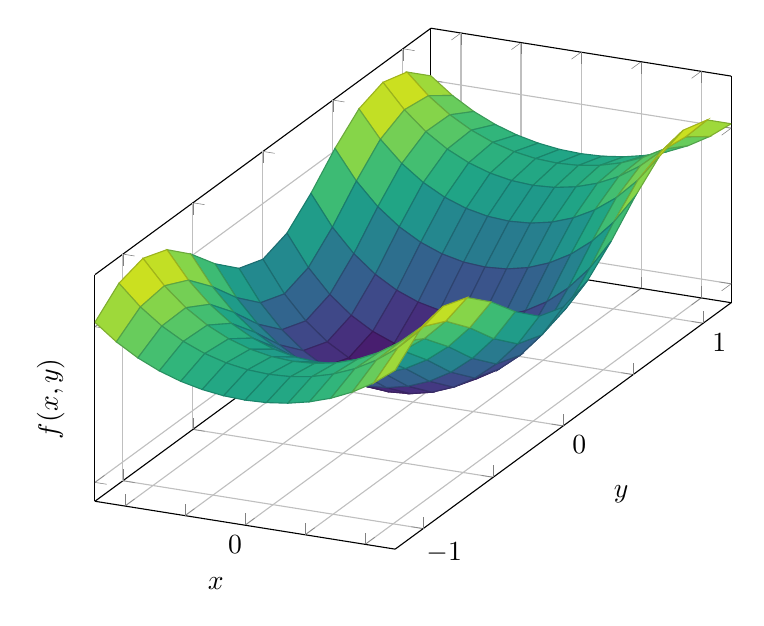
\begin{tikzpicture}
            \begin{axis}[
                colormap name=viridis,
                % 3d box,
                width=15cm,
                view={25}{20},
                axis equal image,
                % enlargelimits=false,
                grid=major,
                domain=-0.5:0.5,
                samples=15,
                yticklabels={,$-1$,,$0$,,$1$},
                xticklabels={,,,$0$},
                zticklabels={,,},
                xlabel=$x$,
                ylabel=$y$,
                zlabel={$f(x, y)$},
                ]
                \addplot3 [y domain = -1.2:1.2, surf]
                    {(x*x+y*y)*exp(x*x-y*y)};
            \end{axis}
        \end{tikzpicture}
    \end{center}

\end{ex}
